\documentclass[11pt]{report}
\usepackage{amssymb} %for Blackboard bold etc
\usepackage{amsmath}
\usepackage{amsfonts}
\usepackage{graphicx} %for including eps graphics
\usepackage{float}
\usepackage[english]{babel}
\usepackage{hyperref}
\usepackage{placeins}

\begin{document}
\title{Reconstruction of Cryo soft X-ray tomographs from B-24 beamline at Diamond Light Source with the TIGRE toolbox}
\author{Ander Biguri}
\maketitle
\chapter*{Introduction}

 %((some description of the data acquisition and what they are doing, plus some acknowledgements))
DISCLAIMER: This is just a technical report that very broadly describes in somehow layman terms the methods and algorithms. It is scientifically and mathematically very vague. I will generate a more serious one once I have feedback from the Diamond team.

Imaging Cryo soft X-rays comes with a series of errors that are hard to control. Due to the low energy use for imaging, the attenuation of the X-rays is strong enough that at some angles the detector barely measures anything. The low energy used also comes with a high scattering and beam hardening effects. Additionally, due to the small size of the samples (in the order of micrometers) there is high misalignment errors (even after correction) and the beam is not 100\% parallel. All this errors lead to highly noisy images, as seen in Figure \ref{fig:TIGREvsIMOD}. Iterative algorithms should, at least, generate less noisy images from the same data, if not better defined images. This technical report describes how these images have been reconstructed with some iterative algorithms. Not all iterative algorithms available in TIGRE have been used. This document shows reconstruction of the dataset named ``2017\_0207\_Trypanosoma\_33''.



In order to compare the reconstructions in TIGRE to a filtered backprojection (FBP), the FBP is recomputed, instead of using the .rec files provided. This is because the .rec files have a different axis of rotation than what TIGRE does, and are the result of an image reconstructed with bigger resolution, and then cropped. All this means that slice-per-slice comparison on the .rec files by IMOD to TIGRE reconstruction will be challenging, as the exact match between them is unknown. Thus, for a better comparison, FBP is recomputed in TIGRE. Both images look very similar, as seen in Figure \ref{fig:TIGREvsIMOD}, where the left corresponds to the IMOD image, the right to TIGRE. Note that the images are similar. The slice is not exactly the same, nor the normalization of the data to the visual range, but finding the perfect one has shown to be very hard. Thus, seeing that TIGREs FBP is almost the same as IMODs, the comparison later will be done using TIGREs version. Note that the IMOD image may look worse than when just loaded from the ``rec'' file but that is just because of the display window. The data shown in the figure is strictly the data loaded from IMOD.



\begin{figure}
\begin{center}

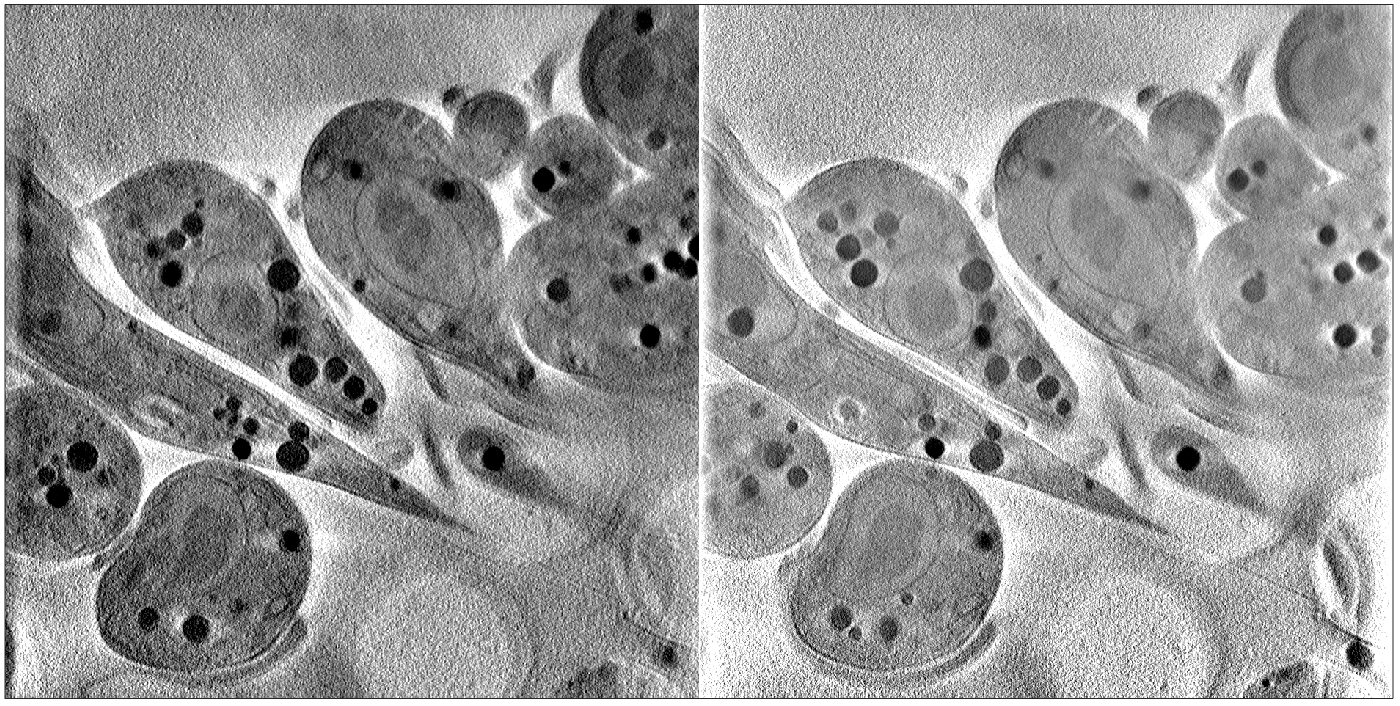
\includegraphics[width=\textwidth]{TIGREvsIMOD.png} 
\end{center}

\caption{\label{fig:TIGREvsIMOD}FBP reconstruction using IMOD (left) and TIGRE (right). This image is inly shown for comparison purposes. Note that the level of noise and extreme image values is similar for both images. TIGRE image is slightly lighter,  due to different normalization than in IMOD (unknown).} 
\end{figure}



Some technical details about the reconstruction process:
\begin{itemize}
\item To reconstruct images with the same contrast as IMOD, a heuristic beam hardening preprocessing step is applied to the data, by squaring the values.
\item The reconstructions have been converted to the 0-255 range heuristically, as I have not found what criteria does IMOD follow for discretization (definitely not min-max nor percentiles). This means that maybe some details will have a different attenuation value than in the FBP example. I can change this discretization as pleased, so if you have any preference let me know.

\item IMODs preprocessing techniques in alineation generate severe artefacts in algorithms that do not update the image using all projections in one go. SIRT, FBP and CGLS update the image in a single update for all data, however most of the other algorithms do use single projections or a small subset of the projections to update the image. This generally means that the latter will get to a better image. However, IMOD aligns the images and fills the regions that are empty with data that is invisible for FBP (because it is zero after a high pass filter) but it is visible for iterative algorithms. See Figure \ref{fig:sino}. Ideally, TIGRE allows detector offsets as an input, thus not needing alineation of the images, however IMOD doesn't seem to output the offset values, only the aligned image. If TIGRE were to be used in a system like this, a separate alineation algorithm would be needed to output the values themselves. That said, for the reconstructions shown here the datasets have been cropped to avoid the data portions generating these artefacts. This also mean that it is very likely that the images are be marginally worse than what they would be when using the full dataset.
\end{itemize}

\begin{figure}
\begin{center}

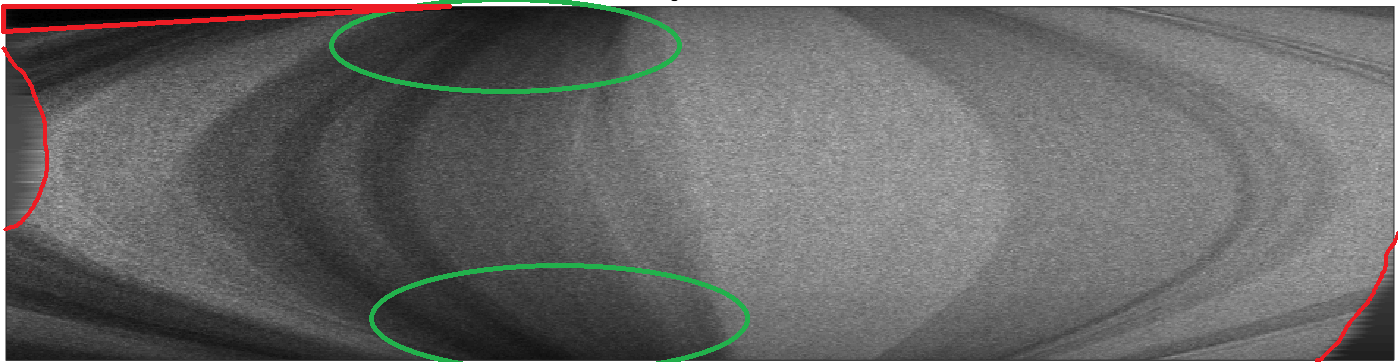
\includegraphics[width=\textwidth]{sinogram.png} 


\end{center}

\caption{\label{fig:sino} Sinogram of the image for the middle row of the detector data. Red areas are artefacts generated by IMOD preprocessing that create errors in TIGRE reconstruction. In green, areas with lower x-ray intensity than what they should have, because the photons attenuated before reaching the detector, also a source of artefacts.} 
\end{figure}




\pagebreak
\chapter*{CLGS and SIRT}
Several algorithms have been used to test the effect of iterative algorithms. Initially SIRT and CGLS have been chosen. Both of these algorithms are expected to generate images with very few noise, but perhaps lose the most detailed information, or at least create smoother boundaries than FBP, as they minimize the L2 norm using all data in one go (per iteration). Result of these, compared to FBP can be seen in Figure \ref{fig:CGLSSIRT}. SIRT generates a very smooth image without barely any noise, however the details are very smoothed also, specially the boundaries of the objects. CGLS however seems to separate data from noise better, while also creating some smooth (not as much as SIRT) boundaries. However it is unclear to me how much of this is caused by misaligments on the data and how much by the algorithms themselves.



\begin{figure}
\begin{center}

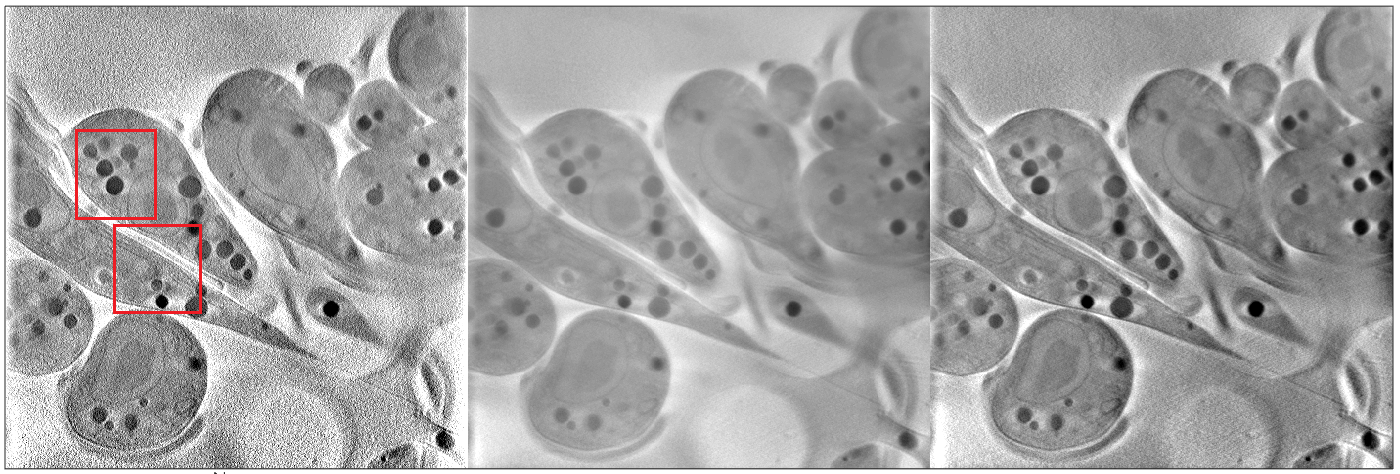
\includegraphics[width=\textwidth]{FBP_SIRT_CGLSm.png} 
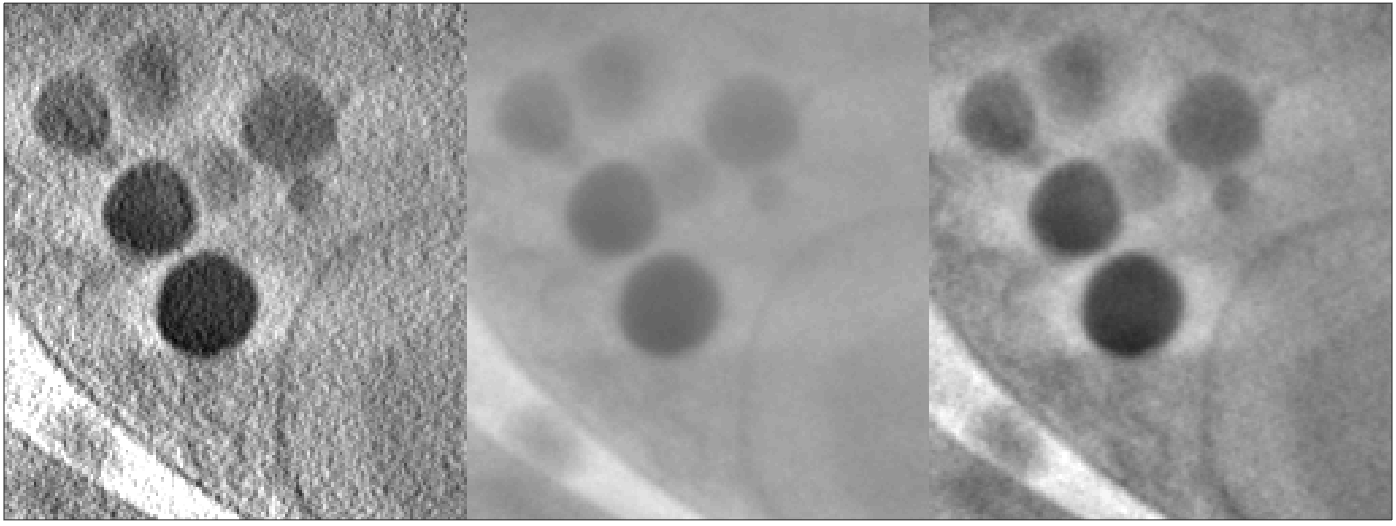
\includegraphics[width=\textwidth]{FBP_SIRT_CGLSz1.png} 
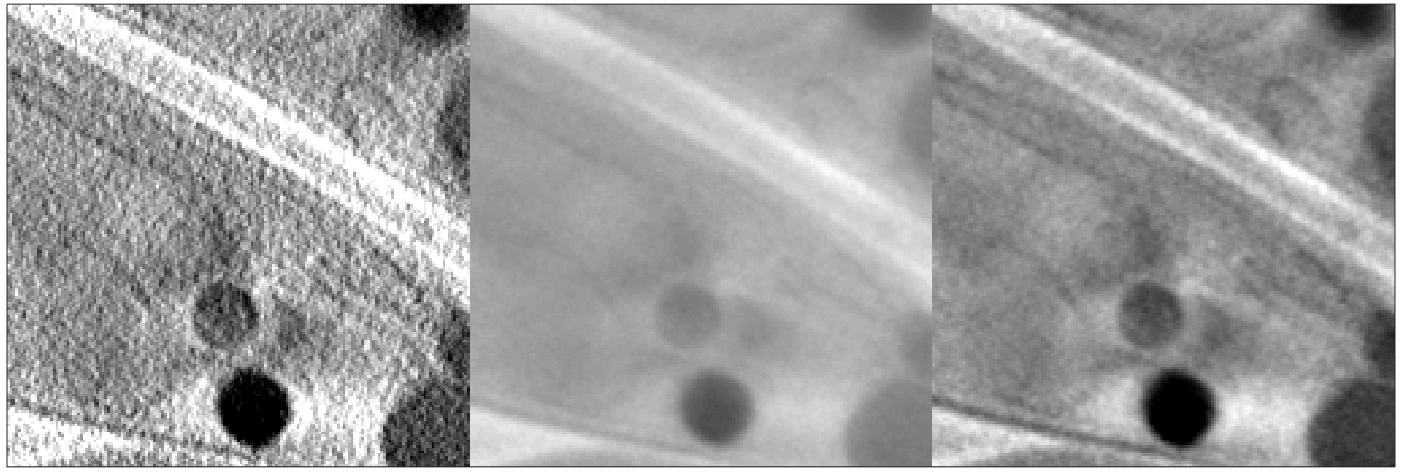
\includegraphics[width=\textwidth]{FBP_SIRT_CGLSz2.png} 

\end{center}

\caption{\label{fig:CGLSSIRT}Columns: FBP, SIRT (20 iterations) and CGLS (7 iterations)} 
\end{figure}

\FloatBarrier

\chapter*{OS-SART and OS-ASD-POCS}
SIRT is an algorithm that updates the image using all the projections in one step. While faster (as each iteration is a single image update), this generally leads to an image that is sometimes too smooth, but definitely not as good as it can be. Think about it as if it averages the errors from all projections, thus creating a smoother image. If for each algorithm iteration the image is updated projection by projection (SART) the information is taken into account ``stronger''. However sometimes that is  both too slow (now each algorithm iteration has as many image updates as projections), and too strict, not removing noise as much as they should. A middle ground option is OS-SART, updating the image several projections at a time. 

Additionally, as the images are very noisy, Total Variation regularization can be added to the algorithm. This adds a constrain to the image reconstruction, by trying to find the image that best fits the data and is more ``flat'' at the same time. The authors called this algorithm ASD-POCS, and OS-ASD-POCS is its OS-SART variation of it. It is basically OS-SART but TV constrained.

The results can be seen in Figure \ref{fig:OS}, where FBP, OS-SART and OS-ASD-POCS are shown. Note that the images have a darker vertical ``band'', not as obvious in SIRT and CGLS. This is caused by the red colored areas on the sinogram of Figure \ref{fig:sino}. OS-SART reconstruct a similar result than FBP, with slightly lower noise levels and extreme values. Les iteration of OS-SART would probably generate a less noisy image, however they will also likely show less contrast and features (similar as SIRT before). The total variation version of OS-SART generates a cleaner image, but it has a slight ``watercolor'' texture. The strength of the total variation can be controlled by the amount of iterations, increasing them enhances this effect. Figure \ref{fig:OStv} shows 0, 20 and 5 TV iterations. While the tuning of this value can not (yet) be done automatically, once the desired one is found it generally works for all similar images.



\begin{figure}
\begin{center}

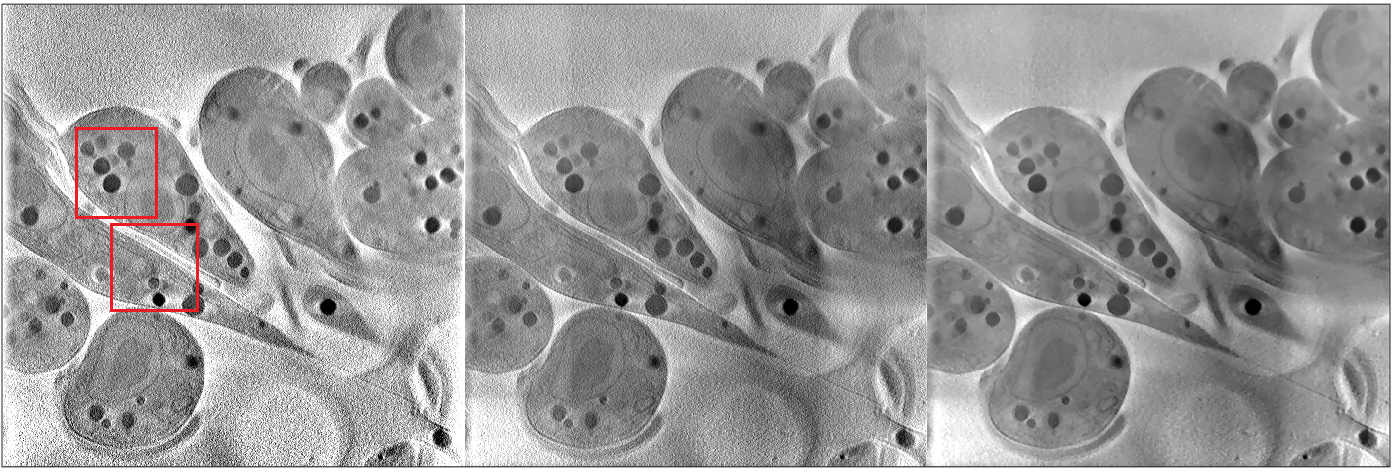
\includegraphics[width=\textwidth]{FBP_OSSART_TV.png} 
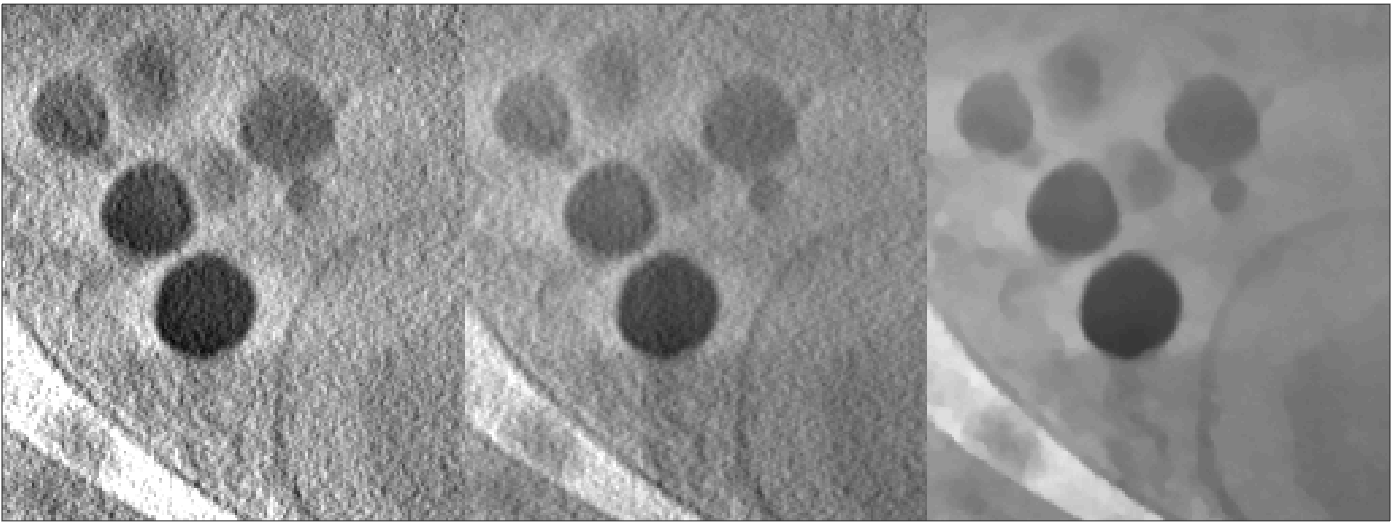
\includegraphics[width=\textwidth]{FBP_OSSART_TVz1.png} 
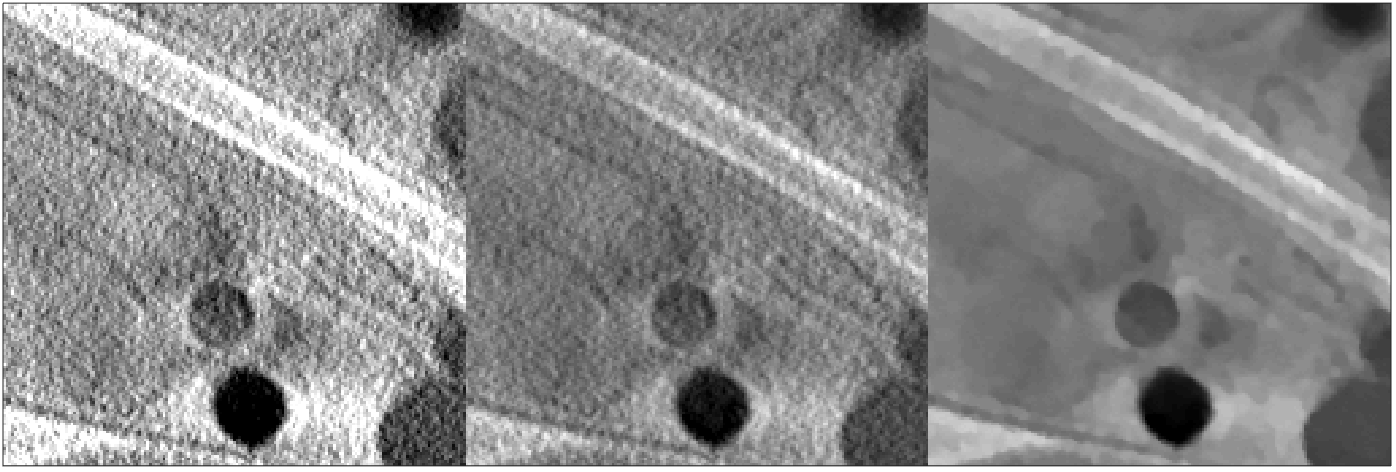
\includegraphics[width=\textwidth]{FBP_OSSART_TVz2.png} 

\end{center}

\caption{\label{fig:OS}Columns: FBP, OS-SART (20 iterations) and OS-ASD-POCS (20 iterations, 20 TV iterations each)} 
\end{figure}


\begin{figure}
\begin{center}

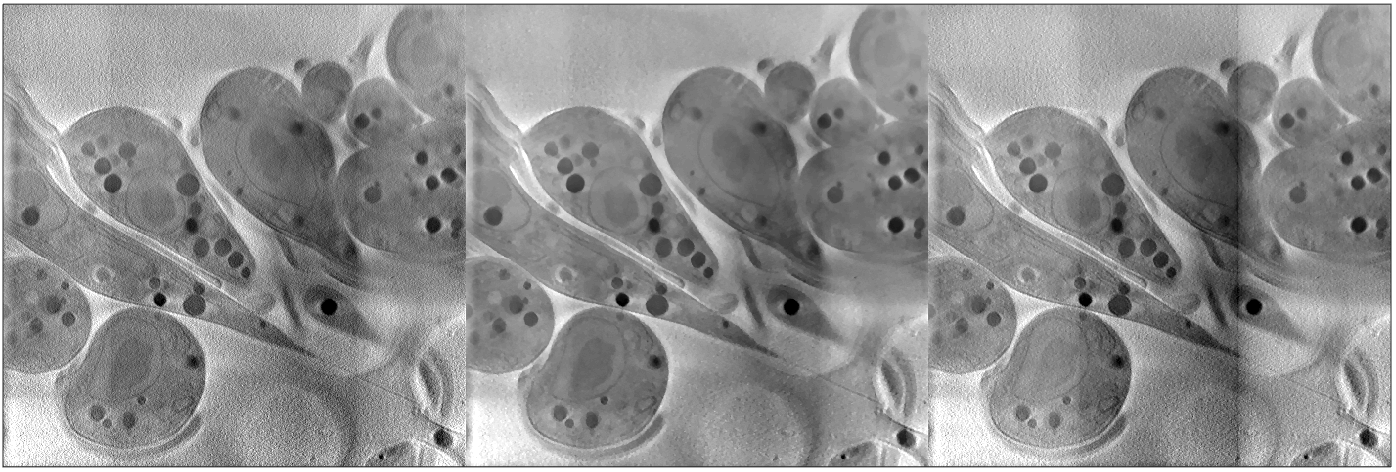
\includegraphics[width=\textwidth]{OSSART_0_20_5_TViters.png} 
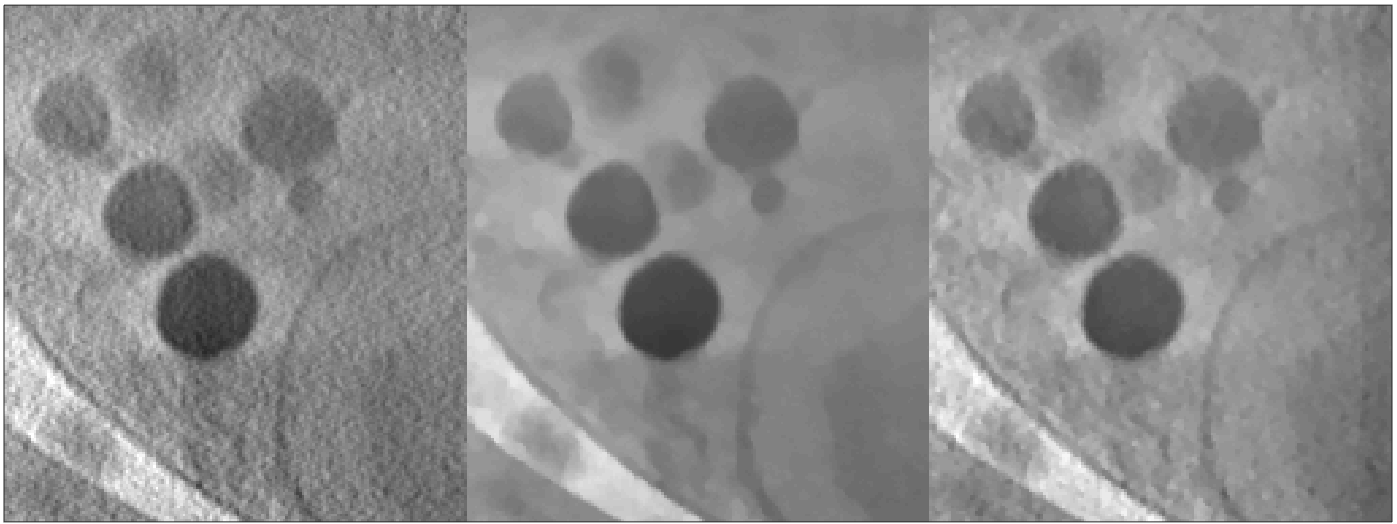
\includegraphics[width=\textwidth]{OSSART_0_20_5_TVitersz1.png} 
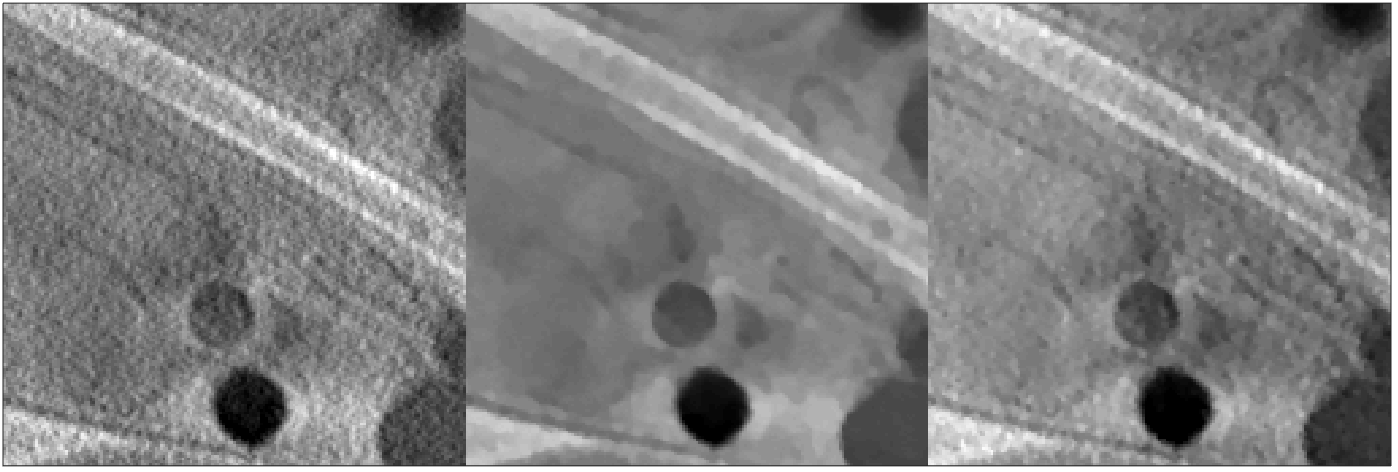
\includegraphics[width=\textwidth]{OSSART_0_20_5_TVitersz2.png} 

\end{center}

\caption{\label{fig:OStv}Columns: OS-SART (20 iterations, 0 TV iterations), OS-ASD-POCS (20 iterations, 20 TV iterations each),OS-ASD-POCS (20 iterations, 5 TV iterations each)} 
\end{figure}


\chapter*{Final remarks}

All reconstructions have been saved in MRC format, trying to match the histogram of the original .rec file, i.e. integer valued of range [-128 127]. If a different discretization or image range is desired, they can be changed as pleased. If comparison between reconstruction is made, I suggest using TIGREs FBP, not IMODs, as the exact same pixel location should correspond to the same object in the image in TIGREs (unlike in IMODs image). Additionally IMOD appears to have a more advanced pre or post processing techniques, thus if the difference between the reconstructions is what is wanted to evaluate, using the same data processing would eliminate other effects. Ideally these pre/post processing techniques could also be applied to TIGRE algorithms to get even better images, unfortunately they are not in TIGRE yet. 

Download link:

 \href{}{https://drive.google.com/open?id=0B4RSIJr6lzdKYVhBdEFnSy1yQUk}
\end{document}